\documentclass[12pt]{article}
\usepackage[hungarian]{babel}
\selectlanguage{hungarian}
\usepackage[utf8]{inputenc}
\usepackage[T1]{fontenc}

\pdfpageheight\paperheight
\pdfpagewidth\paperwidth
\setlength\topmargin{-7mm} \setlength\oddsidemargin{-0cm}
\setlength\textheight{22cm} \setlength\textwidth{15.8cm}
\setlength\columnsep{0.25in}  \newlength\titlebox \setlength\titlebox{2.00in}
\setlength\headheight{5pt}   \setlength\headsep{0pt}
\setlength\footskip{1.9cm}
\setlength\leftmargin{0.0in}

\usepackage{alltt}

\usepackage{tkz-euclide}
\usepackage{tikz}
\usetikzlibrary{shapes.multipart, calc}
\usetikzlibrary{shapes.geometric}
\usetikzlibrary{shapes}
\tikzset{
  treenode/.style = {circle, draw, align=center, inner sep=3pt, text centered, font=\sffamily, text width=1em},
  arn_n/.style = {treenode, circle, white, font=\sffamily\bfseries, draw=black, fill=black, text width=1.5em},
  arn_r/.style = {treenode, circle, red, draw=red, text width=1.5em, very thick}
  rendmint/.style = {rectangle split,rectangle split parts=2,draw,text centered},
  int/.style = {rectangle split,rectangle split parts=2,draw,text centered, text width = 1.6cm, text height = 0.3cm},
  subtree/.style={isosceles triangle, draw=black, align=center, minimum height=0.5cm, minimum width=1cm, shape border rotate=90, anchor=north}
}
\title{1. gyakorlat -- Bináris keresőfák}
\begin{document}

\maketitle

\noindent1. Vegyük az alábbi bináris keresőfát!

\begin{figure}[!h]
\centering
    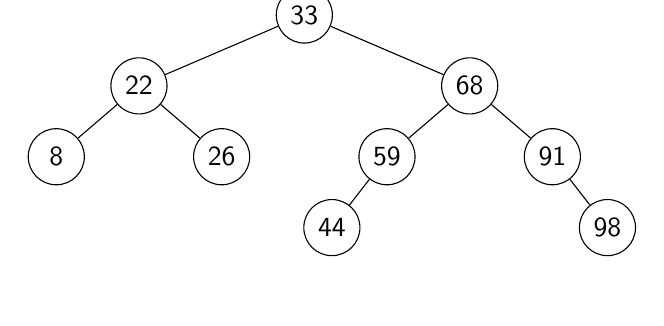
\begin{tikzpicture}[scale=.6, level/.style={sibling distance = 7cm/#1}]
    \node[treenode]{33}
    	child{ node[treenode] {22}
    		child{ node[treenode] {8}}
    		child{ node[treenode] {26}}
    	}
    	child{ node[treenode]{68}
    		child{ node[treenode]{59}
    			child{ node[treenode]{44}}
    			child[missing]
    		}
    		child{ node[treenode]{91}
    			child[missing]
    			child{ node[treenode]{98}}
    		}
    	};
\end{tikzpicture}
\end{figure}

\noindent a) Keressük meg a fában a 11, 89, 44, 90 kulcsokat!

\noindent b) Szúrjuk be a fába a 11, 65, 60 kulcsokat!

\begin{figure}[!h]
\centering
    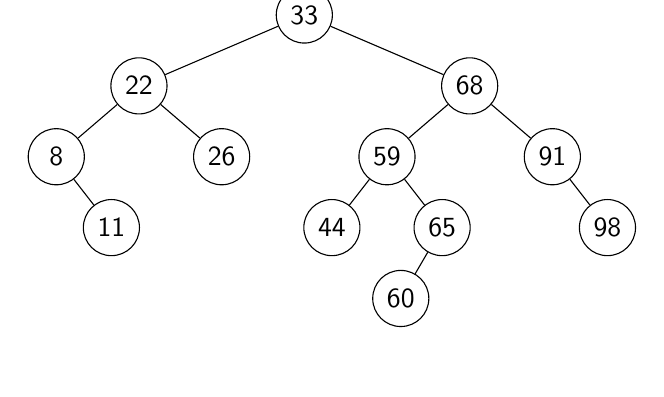
\begin{tikzpicture}[scale=.6, level/.style={sibling distance = 7cm/#1}]
    \node[treenode]{33}
    	child{ node[treenode] {22}
    		child{ node[treenode] {8}
    			child[missing]
    			child{ node[treenode]{11}}    		
    		}
    		child{ node[treenode] {26}}
    	}
    	child{ node[treenode]{68}
    		child{ node[treenode]{59}
    			child{ node[treenode]{44}}
    			child{ node[treenode]{65}
	    			child{ node[treenode]{60}}
    				child[missing]
    			}
    		}
    		child{ node[treenode]{91}
    			child[missing]
    			child{ node[treenode]{98}}
    		}
    	};
\end{tikzpicture}
\end{figure}

\noindent c) Hogyan keresnénk meg egy $r$ gyökerű (rész)fa maximális elemét?

Legkisebb elem: gyökértől kezdve végig jobbra megyünk a fában.

\noindent d) Hogyan keresnénk meg $x$ megelőzőjét?

\begin{enumerate}
\item Ha $x$-nek van bal fia, akkor a bal részfa maximális eleme lesz a megelőző.
\item Ha $x$-nek nincs bal fia, akkor addig megyünk fel a fában, amíg az első $x$-től kisebb kulcsot meg nem találjuk.
\item Ha a gyökérig eljutva sem találunk egyetlen $x$-nél kisebb kulcsot, akkor nem található megelőzője $x$-nek a BKF-ban (vagyis $x$ a fában található legkisebb elem).
\end{enumerate}

Megjegyzés: az előző eljárások értelemszerű módosításával megkaphatjuk az $r$ gyökerű részfa minimális elemét, illetve az $x$ kulcs rákövetkezőjét meghatározó algoritmusokat.

\noindent e) Töröljük a beszúrások után előálló fából a 26, 8, 68 kulcsokat!

\begin{figure}[!h]
\centering
    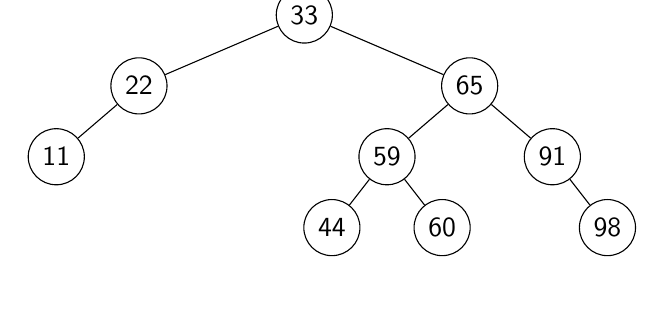
\begin{tikzpicture}[scale=.6, level/.style={sibling distance = 7cm/#1}]
    \node[treenode]{33}
    	child{ node[treenode] {22}
    		child{ node[treenode] {11}}
			child[missing]
    	}
    	child{ node[treenode]{65}
    		child{ node[treenode]{59}
    			child{ node[treenode]{44}}
    			child{ node[treenode]{60}}
    		}
    		child{ node[treenode]{91}
    			child[missing]
    			child{ node[treenode]{98}}
    		}
    	};
\end{tikzpicture}
\end{figure}

\noindent2. Tegyük fel, hogy egy bináris keresőfában a 15-ös elemet keressük. Lehetséges keresési sorozat-e az alábbi: 20, 9, 12, 8, 15?

Nem, ugyanis 15 nagyobb, mint a 12, ezért a 8-as a 12 jobb fia kellett, hogy legyen, de ez ellentmondás, hiszen a 12 jobb részfájában nem lehetnek nála kisebb elemek.

\noindent3. Írassuk ki a fa elemeit kulcs szerint növekvő sorrendben!

\begin{alltt}
      void inorder(x) \{
        if(x!=nil) \{
          inorder(x.bal);
          print(x.kulcs);
          inorder(x.jobb);
        \}
      \}
\end{alltt}

\noindent4. Szúrjuk be egy üres bináris keresőfába a következő elemeket a megadott sorrendben: 1,2,3,4,5,6,7

\begin{figure}[!h]
\centering
    \begin{tikzpicture}[scale=.6, level/.style={sibling distance = 3cm}]
    \node[treenode]{1}
		child[missing]
    	child{ node[treenode] {2}
			child[missing]
    		child{ node[treenode] {3}
				child[missing]
    			child{ node[treenode] {4}
					child[missing]
	    			child{ node[treenode] {5}
						child[missing]
		    			child{ node[treenode] {6}
							child[missing]
			    			child{ node[treenode] {7}}
		    			}
	    			}
    			}
    		}
    	};
\end{tikzpicture}
\end{figure}

\end{document}